\documentclass[tikz,border=10pt]{standalone}
\usepackage{amsmath}
\begin{document}
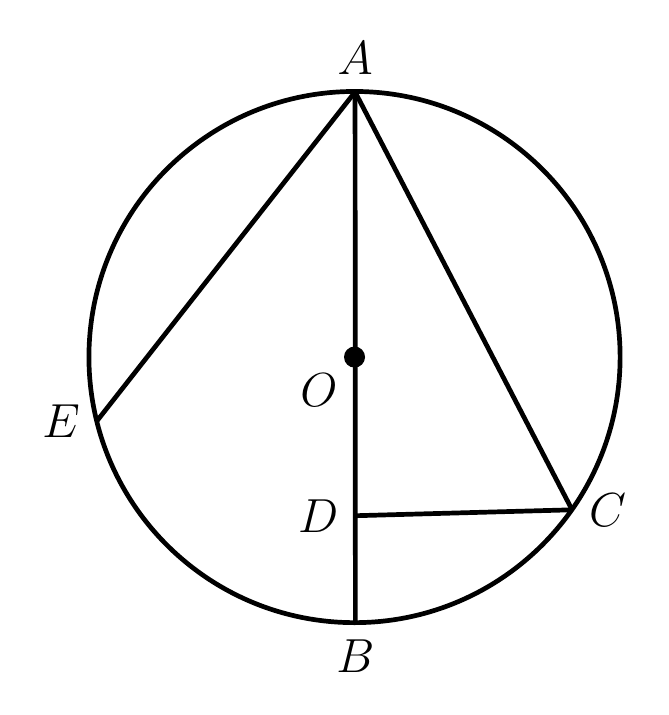
\begin{tikzpicture}[line join=round, line width=1.7pt]
\coordinate (A) at (0.253,3.383);
\coordinate (B) at (0.257,-3.357);
\coordinate (C) at (3.009,-1.924);
\coordinate (D) at (0.257,-1.999);
\coordinate (O) at (0.246,0.016);









\coordinate (E) at (-3.028,-0.799);


\draw (O) circle (3.373);


\draw (A) -- (B);
\draw (A) -- (E);
\draw (A) -- (C);
\draw (C) -- (D);


\fill (O) circle (3.800pt);


\fontsize{18}{21.6}\selectfont
\node[above] at (A) {$A$};
\node[below] at (B) {$B$};
\node[right] at (C) {$C$};
\node[left] at (D) {$D$};
\node[below left] at (O) {$O$};
\node[left] at (E) {$E$};
\end{tikzpicture}
\end{document}